% !TEX encoding = UTF-8 Unicode
% !TEX TS-program = latexmk
\documentclass[french]{scrartcl}%<1
\usepackage[utf8]{inputenc}
\usepackage[T1]{fontenc}
\usepackage{lmodern}
\usepackage{microtype}
\usepackage{tikz,calc}
%\usepackage[arrows=false]{pagegrid}
\usetikzlibrary{patterns,patterns.meta}

% A\c c = 210mm x 297mm
\newlength{\MLsurfacelargeur}\setlength{\MLsurfacelargeur}{180.0000mm}
\newlength{\MLsurfacehauteur}\setlength{\MLsurfacehauteur}{264.0000mm}
\newlength{\MLmargehaut}\setlength{\MLmargehaut}{16.50000mm}
\newlength{\MLmarge}\setlength{\MLmarge}{13.50000mm}
\newlength{\MLmargeinterne}\setlength{\MLmargeinterne}{210.00000mm-\MLsurfacelargeur-\MLmarge-\MLmarge+2mm}
\newlength{\MLmargegauche}\setlength{\MLmargegauche}{\MLmarge+\MLmargeinterne}
\newlength{\MLbarrehaut}\setlength{\MLbarrehaut}{18.00000mm}
\newlength{\MLbarrebas}\setlength{\MLbarrebas}{\MLsurfacehauteur-42.00000mm}
\newlength{\MLbarrevert}\setlength{\MLbarrevert}{50.00000mm}
\newlength{\ML}\setlength{\ML}{0mm}

\usepackage[%
%	showframe, showcrop,
	paper=a4paper,
	layout=a4paper,
	marginparsep=0mm,
	marginparwidth=0mm,
	headsep	=25.00000mm,
	footskip	=59.00000mm,
	top		=37.00000mm,
	inner		=66.50000mm,
	width		=130.00000mm,
	height	=191.5000mm,
	]{geometry}
%\usepackage{layout} % \newpage\layout*

\newlength\tindent % pour un indent manuel
\setlength{\tindent}{\parindent}
\setlength{\parindent}{0pt}
\renewcommand{\indent}{\hspace*{\tindent}}
\pagestyle{empty}
\usepackage{babel}
\newcommand\myrlc{\hspace{17.1mm}}
\newcommand\trou{%
	\draw (9.00000mm, -28.00000mm) circle (3.00000mm) ;%
	\draw (9.00000mm,-108.00000mm) circle (3.00000mm) ;%
	\draw (9.00000mm,-188.00000mm) circle (3.00000mm) ;%
	\draw (9.00000mm,-268.00000mm) circle (3.00000mm) ;%
}
\newcommand\watermark{\node[anchor=mid,rotate=90] at (-3.00000mm,-211.00000mm) {{\tiny cyril.rouiller@edufr.ch}};}

\begin{document}%<1

\begin{tikzpicture}[remember picture,overlay,shift=(current page.north west)]
	\begin{scope}[shift={(\MLmargegauche,-\MLmargehaut)}] % point superrieur gauche de la zone de travail
		\draw[black!100,thick] (0,0) rectangle (\MLsurfacelargeur,-\MLsurfacehauteur);% cadreextérieur
		\draw[gray!30, thin] (0,0) grid[step=4.00000mm] (\MLsurfacelargeur,-\MLsurfacehauteur);% grille
		\draw (0,-\MLbarrehaut) --+ (\MLsurfacelargeur,0);% barre du haut
		\draw (0,-\MLbarrebas) --+ (\MLsurfacelargeur,0);% barre du bas
		\draw (\MLbarrevert,-\MLbarrehaut) --+ (0,-\MLbarrebas+\MLbarrehaut);% barre verticale
		\node[left,baseline] at ( 17mm,  -6.0mm) {Nom :};
		\node[left,baseline] at (105mm,  -6.0mm) {Date :};
		\node[left,baseline] at (157mm,  -6.0mm) {Page :};
		\node[left,baseline] at ( 17mm, -13.9mm) {Matière :};
		\node[left,baseline] at (105mm, -13.9mm) {Chapitre :};
%	\watermark
%		\node[left,baseline] at (165mm, -262mm){{\footnotesize Relecture : 1)\myrlc 2)\myrlc 3)\myrlc 4)\myrlc 5)}};
%		\node[right,baseline] at ( 17mm,  -6.0mm) {NOM Prénom};
%		\node[right,baseline] at (105mm,  -6.0mm) {\today};
%		\node[right,baseline] at (157mm,  -6.0mm) {1};
%		\node[right,baseline] at ( 17mm, -13.9mm) {Branche traitée};
%		\node[right,baseline] at (105mm, -13.9mm) {Thématique};

	\end{scope}
	\trou
\end{tikzpicture}

\end{document}%<1
% vim: set ts=3 sts=3 sw=3 tw=100 fdm=marker foldmarker=%<,%> filetype=tex spell:%
